{$\space$\par}
\vspace{0.5cm}
\justifying
\section*{\bfseries \LARGE Questão 5 - \large A galáxia NGC 5548 hospeda um AGN classificado como Seyfert 1. Peterson et al. (1999) observaram seu fluxo durante 8 anos no contínuo óptico (em 5100 Å) e na linha H$\beta$. O arquivo \texttt{NGC5548.dat} contém a data juliana da observação (JD), os fluxos no contínuo óptico e na linha H$\beta$ (F5100 e FHbeta), bem como seus respectivos erros (e\_F5100 e e\_FHbeta). Os fluxos estão medidos em erg cm$^{-2}$ s$^{-1}$ Å$^{-1}$.}

\vspace{0.3cm}

\begin{enumerate}
    \item Suponha que seja possível descrever o fluxo no contínuo óptico deste AGN a partir do fluxo na linha H$\beta$, e que apenas essas duas informações sejam conhecidas. Que parametrização seria essa?
        
    \item Suponha agora que as medidas de erro sejam conhecidas. Critique o resultado obtido acima com base no que esses erros indicam. Represente ambas as distribuições empíricas em um gráfico quantil-quantil.

    \item Conhecendo os valores medidos para os fluxos e seus erros estimados, sugira uma parametrização mais adequada. Explique por que ela é mais adequada a esse problema e como ela foi obtida. 
\end{enumerate}
\vspace{0.8cm}

\textcolor{red}{A) Essa parametrização seria uma regressão linear ordinária, onde não leva-se em conta possíveis erros nas variáveis dependente e independente. Para isso, usei o linear model (lm) do R.}

\vspace{0.8cm}

\begin{lstlisting}
    ngc = read.table('/content/NGC5548.dat', sep='|', header = T)
    ngc = ngc[complete.cases(ngc),]
    
    options(repr.plot.width=10,repr.plot.height=10)
    
    fit = lm(F5100 ~ FHbeta, data = ngc)
    
    x_vals = seq(min(ngc$FHbeta), max(ngc$FHbeta), length.out = 200)
    y_pred = predict(fit, newdata = data.frame(FHbeta = x_vals))
    
    plot(ngc$FHbeta, ngc$F5100, pch=20, xlab="FHbeta", ylab="F5100",
    xlim=c(6,14), ylim=c(7,15))
    lines(x_vals, y_pred, col = "blue", lwd = 2)
    
    for (i in 1:length(ngc$FHbeta)) {
      lines(
        c(ngc$FHbeta[i], ngc$FHbeta[i]),
        c(ngc$F5100[i] + ngc$e_F5100[i], ngc$F5100[i] - ngc$e_F5100[i]),
        col=gray(0.5)
        )
      lines(
        c(ngc$FHbeta[i] + ngc$e_FHbeta[i], ngc$FHbeta[i] - ngc$e_FHbeta[i]),
        c(ngc$F5100[i], ngc$F5100[i]),
        col=gray(0.5)
        )
    }
\end{lstlisting}


\begin{figure}[h]
    \centering
    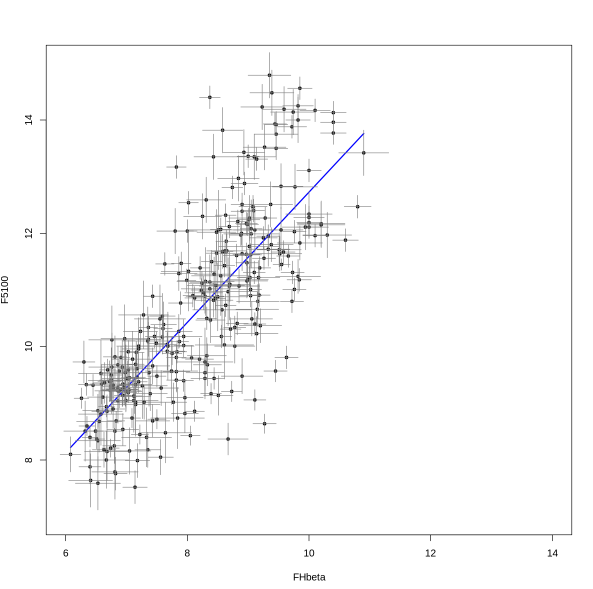
\includegraphics[width=0.6\linewidth]{Figuras/fit_a.png}
    \caption{Regressão linear ordinária do fluxo contínuo no ótico em relação ao fluxo na linha H$\beta$ em azul. Os pontos mostram os dados com as barras de erro.}
    \label{fit_a}
\end{figure}


\textcolor{red}{B) Se as medidas de erro são conhecidas, então devemos utilizar um método que leve em conta possíveis erro nas medidas. Além disso, deve-se usar a variável com menor erro como variável independente e para verificar qual tem menor erro, eu calculei o RMS do erro relativo de ambas quantidades. Logo, deve-se utilizar o fluxo em contínuo no ótico como variável independente.}

\begin{lstlisting}
    rms_rel_F5100 = sqrt(mean((ngc$e_F5100 / ngc$F5100)^2))
    rms_rel_FHbeta = sqrt(mean((ngc$e_FHbeta / ngc$FHbeta)^2))
    
    cat("Erro RMS relativo em F5100:", round(rms_rel_F5100, 3), "\n")
    cat("Erro RMS relativo em FHbeta:", round(rms_rel_FHbeta, 3), "\n")

    ### output ###
    Erro RMS relativo em F5100: 0.033 
    Erro RMS relativo em FHbeta: 0.034 
\end{lstlisting}

\textcolor{red}{C) A parametrização mais adequada para esse caso é o método de mínimos quadrados pesado pelo erro e utilizando o valor com menor erro como variável independente. Para isso, usei o linear model (lm) usando os erros como peso.}

\begin{lstlisting}
    weight = 1 / (ngc$e_FHbeta * ngc$e_FHbeta)
    
    fit = lm(FHbeta ~ F5100, data = ngc, weights = weight)
    
    x_vals = seq(min(ngc$F5100), max(ngc$F5100), length.out = 200)
    y_pred = predict(fit, newdata = data.frame(F5100 = x_vals))
    
    plot(ngc$F5100, ngc$FHbeta, pch = 20, ylab = "FHbeta", xlab = "F5100",
    ylim=c(6,14), xlim=c(7,15))
    lines(x_vals, y_pred, col = "blue", lwd = 2)
    
    for (i in 1:nrow(ngc)) {
      lines(
        c(ngc$F5100[i] - ngc$e_F5100[i], ngc$F5100[i] + ngc$e_F5100[i]),
        c(ngc$FHbeta[i], ngc$FHbeta[i]),
        col = gray(0.5)
      )
      
      lines(
        c(ngc$F5100[i], ngc$F5100[i]),
        c(ngc$FHbeta[i] - ngc$e_FHbeta[i], ngc$FHbeta[i] + ngc$e_FHbeta[i]),
        col = gray(0.5)
      )
    }
\end{lstlisting}

\begin{figure}[h]
    \centering
    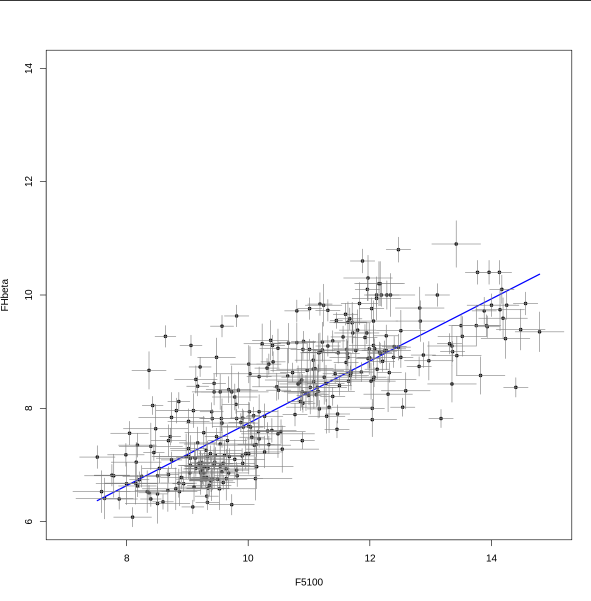
\includegraphics[width=0.6\linewidth]{Figuras/fit_b.png}
    \caption{Regressão linear pesada pelo erro do fluxo na linha H$\beta$ em relação ao fluxo contínuo no ótico em azul. Os pontos mostram os dados com as barras de erro.}
    \label{fit_b}
\end{figure}